\subsection{Problema 5}

\textit {“Realice un algoritmo para determinar cuánto pagará una persona que adquiere N artículos, los cuales están de promoción. Considere que si su precio es mayor o igual a \$200 se le aplica un descuento de 15\%, y si su precio es mayor a \$100 pero menor a \$200, el descuento es de 12\%; de lo contrario, sólo se le aplica 10\%. Se debe saber cuál es el costo y el descuento que tendrá cada uno de los artículos y finalmente cuánto se pagará por todos los artículos obtenidos.”}

\textbf{Paso 1: Creación de archivos y definición de modelos}

Se crearon diferentes archivos .dart para la solución del problema dentro de los archivos se crearon: 
\begin{itemize}
    \item articulo\_controller.dart
    \item articulo\_model.dart
    \item articulo\_view.dart
    \item articulo\_card.dart
\end{itemize}

\textbf{articulo\_model.dart}

En el primero archivo que es articulo\_model.dart se definió la estructura de datos de un artículo o productos dentro de la app que se desarrollo para resolver el problema. Dentro del archivo se creó la clase ArticuloModel que tiene algunos atributos como el precio, el descuento que va a recibir y el total, además dentro de esta clase se crea una funcio llamada calcular esta es la que permite construir un articulo completo con el precio orginal, el código de forma genera lo que hace es definir el porcentaje de descuento que se va aplicar atraves de sentencias Ifs anidades, también hace los cálculos del monto de descuento en dólares que va a tener un articulo y también hace la respta respectiva del precio  - descuento para poder obtener el valor final aplicado el descuento, al final esta clase empaqueta los 3 atributos en un objeto llamado articulo.


\begin{center}
\begin{lstlisting}
class Articulo {
  final double precio;
  final double descuento;
  final double total;

  Articulo({
    required this.precio,
    required this.descuento,
    required this.total,
  });
\end{lstlisting}
\end{center}

\textbf{articulo\_controller.dart}

Después en el archivo, se utilizo el respectivo modelo ya creado en esta se crea una clase llamada ArticuloController en la cual se crea una lista privada a la cual se le llamo \_artículos aquí se guardan los artículos que se van agregando dentro de la aplicación, esta case tiene algunas funciones principales entre estas las mas importantes son agregar artículos la cual trabaja con el modelo internamiente esta llama a Articulo.calcular con esta función se devuelve un objeto completa con su precio y descuento ya calculado dentro del modelo, y el controlador añade el arituclo a lista \_artículos, otra función importante es calcularTotal la cual revisa y toma todos los artículos que se guardan en la lista, de cada uno de los arituculos almacenados en la lista se va sumando el total que es el valor con el descuento aplicado y suma estos valores para devolver el total de la compra o de todos los artículos que se registran en la lista, otra función importante es limpiar la cual vacia la lista borrando todos los artículos que se agregaron en la lista.


\begin{center}
\begin{lstlisting}
  final List<Articulo> _articulos = [];
  
  List<Articulo> get articulos => _articulos;
  
  void agregarArticulo(double precio) {
    _articulos.add(Articulo.calcular(precio));
  }
  void limpiar() {
    _articulos.clear();
  }
  double calcularTotal() {
    return _articulos.fold(0, (sum, item) => sum + item.total);
  }
\end{lstlisting}
\end{center}

\textbf{articuloCard}

El archivo se creo con el propósito de poder dibujar una Tarjeta que permita mostrar un articulo considerando que se va a guardar como un objeto, la idea de esta clases es que poder mostrar los artículos para esto utiliza el modelo es por medio del modelo por el que recibe un objeto Articulo y de este se saca el precio, descuento y el total, para la tarjeta se usa la librería que se importa, por lo que no se utilizan colores estándar de flutter, si no que se definieron colores definidos dentro de nuestro proyecto para trabajar con un paleta de colores definida en todos los problemas, algo adicional que se hace en esta clase es que se calcular el porcentaje de descuento para mostrar en la tarjeta.

\textbf{articulo\_view.dart}

Por ultimo en el archivo, aquí es donde se unen los códigos anteriores, para poder crear la interfaz final que se va a mostrar al usuario final dentro de este archivo se crea un StatefulWidget, la cual permite hacer una actualización cada ves que se ingresa un nuevo producto, de forma general tiene cuatro partes importantes, la Entrada de datos el cual muestra un campo de texto con un UltraInput para poder ingresar el precio y también muestra el botón para agregar y limpiar artículos, después se tiene la lista de artículos que es la parte principal esta revisa los artículos del controller y si no se tiene artículos se muestra el mensaje “No hay artículos agregados”, pero si la lista tiene artículos se usa un ListView.builder para crear un ArticuloCard por cada uno de los artículos que se tenga en la lista del controlador, otra parte importante de la View es el Resumen total el cual llama de forma constante a controlle.calcularTotal que muestra el total a pagar por cada articulo agregado, este valor se actualiza, y por ultimo se tiene una gestión de estados y de lógica de forma resumida se crea una instancia de ArticuloController la cual se usa para guardar el estado de la aplicación, también se tiene la lógica del botón agregar en la cual se valida que el numero sea valido caso contrario mostrara un error y si es valido se llama a controller.agregarArticulo, también se tiene la lógica del botón de limpiar para poder eliminar los artículos de la lista, algo importante dentro de la lógica de los botones es el setState la cual cada ves que se presiona se vuelve a graficar la pantalla o se actualiza para poder mostrar los artículos actualizados tanto si se limpiaron o si se agregaron.


\textbf{Paso 4: Integración en la aplicación}

Una ves que se programo una solución utilizando la metodologia atomic design y el patron MVC para el problema se procedio a instanciar en el main.dart y en el home.dart que permiten la navegación entre los programas y también mostrar el la plantilla que se creo. 

Lo primero que se realizo, en main.dart es importar el package que corresponde a products, específicamente la vista articulo\_view.dart, para de esta forma poder instanciarla en el MaterialApp. Después, se registra la ruta por su nombre '/articulos', esto se realiza  dentro del routes del MaterialApp, y de esta forma se asocia al widget ArticuloView, de tal forma que permite la navegación mediante rutas nombradas.

Despues en el archivo home.dart, lo que se realizo es la modificación el quinto HomeButton para cambiar el ícono a Icons.calculate\_rounded que de alguna manera interpreta una calculardora que tiene algo de relación con el problema. Además también, en el método onClick, se utilizo Navigator.pushNamed para definir la navegacion con nombres de ruta para este se define '/articulos', de esta forma al presionar el botón, el usuario va a navegar hacia la pantalla ArticuloView.

De esta manera, se logra integrar la nueva funcionalidad de cálculo de promociones en la aplicación, asegurando que el Home actúe como menú central y la navegación sea clara, directa y reutilizable.


\begin{center}
\begin{lstlisting}
// MAIN
'/products': (context) => const ArticuloView(),

// HOME  
icon: Icons.calculate_rounded,
title: "Promociones",
onClick:  () => Navigator.pushNamed(context, '/products'),
\end{lstlisting}
\end{center}

\textbf{Paso 5: Pruebas y verificación}

Por ultimo para verificar el funcionamiento se realizaron algunas pruebas ingresando diferentes valores 250 - 150 - 100 - 50 y al final todos los resultados fueron correctos.

\begin{figure}[H]
    \centering
    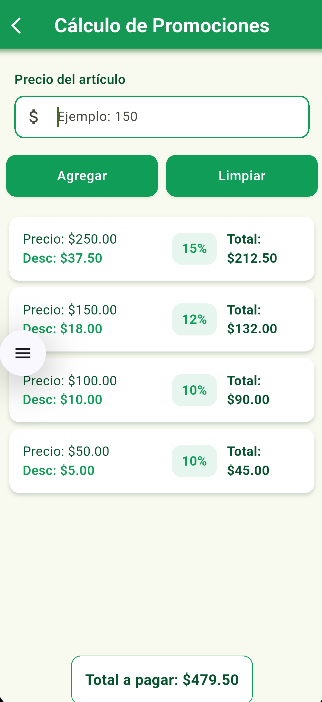
\includegraphics[width=0.6 \textwidth, height=8cm, keepaspectratio]{ejecucion_ej5.png}
    \caption{Verificación ejercicio 5}
    \label{fig:ej5_ejecuccion}
\end{figure}
